\documentclass[a4aper,12pt]{report}
\usepackage[margin=1in]{geometry}
%For Drawing 
\usepackage{tikz}
\usetikzlibrary{intersections}
\usetikzlibrary{shapes.geometric, arrows}
\usepackage[american,RPvoltages]{circuitikz}
\ctikzset{
    resistors/scale=0.6    
}
%For image
\usepackage{graphicx}
\usepackage{changepage} 
%Hyperlinking Texts and Others
\usepackage{hyperref}
\hypersetup{
    colorlinks = true,
    linkcolor=black,
    urlcolor=black,
    pdftitle = {EEE-2103: Digital Electronics }
}
%Header and Footer
\usepackage{fancyhdr}
\pagestyle{fancy}
\lhead{EEE-2101: Analog Electronics I}
\rhead{Note by \href{https://www.facebook.com/mdgalibashrafbd}{Md. Galib Ashraf}}

\usepackage{gensymb}
\usepackage{fancyvrb}
\usepackage{lipsum}

%For creating boxes and others fancy
\usepackage[most]{tcolorbox}
\tcbuselibrary{listings, breakable}
% Define custom tcolorbox style for question and solution
\newcounter{questionbox}[chapter]
\renewcommand{\thequestionbox}{\thechapter.\arabic{questionbox}}
\newtcolorbox{questionbox}[1][]{
  title=\textbf{Q~\thequestionbox:} ~#1,
  coltitle=black,
  colback=black!5,
  colframe=black!75!white,
  colbacktitle=black!80,
  coltitle=white, 
  breakable,
  enhanced,
  rounded corners,
  boxrule=1pt,
  left=8pt,
  right=8pt,
  top=6pt,
  bottom=6pt,
  before upper={\stepcounter{questionbox}}
}
\newcounter{examplebox}[chapter]
\renewcommand{\theexamplebox}{\thechapter.\arabic{examplebox}}

% Define the example box
\newtcolorbox{examplebox}[1][]{
  title=\textbf{Example~\theexamplebox:}~#1,
  coltitle=white,
  colback=blue!5,
  colframe=blue!60!black,
  colbacktitle=blue!30!black,
  breakable,
  enhanced,
  boxrule=1pt,
  arc=4pt, % custom curvature for difference
  top=6pt,
  bottom=6pt,
  left=8pt,
  right=8pt,
  before upper={\stepcounter{examplebox}}
}
% Simple theorem-style box with no title
\newtcolorbox{theorembox}[1][]{
  colback=blue!5,
  colframe=blue!80!black,
  boxrule=0.8pt,
  sharp corners,
  breakable,
  left=8pt,
  right=8pt,
  top=6pt,
  bottom=6pt,
  before upper={\IfNoValueTF{\textbf{#1} // /quad}{\textbf{Default theorem statement goes here.}}{#1}}
}


%To add color in texts
\usepackage{xcolor}

%For using correct symbols and others by default
\usepackage{amsmath, amssymb, amsfonts}

%For Styling Chapters title
%Options: Sonny, Lenny, Glenn, Conny, Rejne, Bjarne, Bjornstrup
\usepackage[Conny]{fncychap}

\usepackage{enumitem}
%for multiple columns 
\usepackage{multicol}

\usepackage{array,tabularx}
\usepackage{colortbl}
\renewcommand{\arraystretch}{1.5}
\begin{document}
    \begin{center}
        \begin{Large}
            \textbf{\noindent Department of Electrical and \\ Electrronics Engineering} \\
        \end{Large}
        \begin{large}
            University of Dhaka \\
        Batch - 103, EEE-58 \\
        \end{large}
        \vspace{0.5cm}
        \begin{large}
            $2^{nd}$ Year $1^{st}$ Semester \\ 
        \end{large}
        \vspace{0.5cm}
        
\includegraphics[scale=0.35]{logo.du.png} \\
        \vspace{0.5cm}
    \end{center}

        \noindent\textbf{Course: EEE-2103} \\ 
        \textbf{Title: Digital Electronics}\\
        Class Techer: Dr. Sharnali Islam\\
    \vspace{0.5cm}
    \begin{center}
            Note by \\
        Md. Galib Ashraf \\
        Session: 2023-2024 \\ 
        Class Roll: SH-042
    \end{center}
    \thispagestyle{empty}
    \newpage 
    \chapter*{Syllabus}
    \thispagestyle{empty}
    \vspace*{-2.7cm}
   \textbf{Introductory Concepts:} Digital and Analog Quantities, Binary Digits, Logic Levels, Digital Electronic Signals and Switches, Basic Logic Functions, Combinational and Sequential Logic Functions, Introduction to Programmable Logic and Fixed-Function Logic Devices. \\ [5pt]
   \textbf{Number Systems, Operations, and Codes:} Decimal, Binary, Hexadecimal, Octal and Binary Coded Decimal Number Systems, Binary Arithmetic and Digital Codes. \\ [5pt]
   \textbf{Logic Gates:} Inverter, AND Gate, OR Gate, NAND Gate, NOR Gate, ExclusiveOR and Exclusive-NOR Gate, Universal Gate, Programmable Logic, FixedFunction Logic Gates. \\ [5pt]
   \textbf{Boolean Algebra and Logic Simplification:} Boolean Operations, Expressions,Laws and Algebra, De Morgan’s Theorems, Boolean Analysis of Logic Circuits, The Karnaugh Map, Don’t Care Conditions, SOP and POS Minimization. \\[5pt]
   \textbf{Arithmetic Operations and Circuits:} Half and Full Adders, Half and Full Subtractor, 2’s complement, Ripple Carry and Look-Ahead Carry Adders, BCD Adders, Cascading BCD Adders, Multipliers. \\ [5pt]
   \textbf{Functions of Combinational Logic:} Decoders: 1-of-8 decoders, BCD-to-Decimal Decoder/Driver, BCD-to-7-Segment Decoder/Drivers, Decoder IC, Encoders and Applications, Priority Encoders, Code Converters, Magnitude Comparators, Parity.Generators/Checkers, Multiplexers: Two, Four, Eight, Sixteen, Quad Two-Input MUX, Multiplexer Applications: Data Routing, Parallel-to-Serial Conversion, Logic Functions Generation, Demultiplexers and its Applications, 1-Line-to-8-Line Demultiplexer, Synchronous Data Transmission. \\ [5pt]
   \textbf{Sequential Logic:} NAND/NOR Gate Latch, Edge-Detector Circuit, Flip-Flops: Clocked S-C Flip-Flop, Clocked J-K Flip-Flop, Clocked D Flip-Flop, T Flip-Flop, Master/Slave Flip-Flop, Clocked J-K Flip-Flop with Asynchronous Inputs, FlipFlop Applications: Edge Detection, Switch Bouncing Reduction, Parallel Data Transfer, Serial Data Transfer. Shift Registers and Counters: Shift Register Operations, Types of Shift Register, Shift Register Counters: Ring Counter and Johnson Counter, Asynchronous Counters, IC Asynchronous Counters, Asynchronous Down Counters, Synchronous Up/Down Counters, Pre-settable Counters, Counter with Arbitrary Sequences, Design of Synchronous Counters and Cascaded Counters. \\ [5pt] 
   \textbf{Interfacing with the Analog World:}Methods of Digital-to-Analog Conversion: Weighted Resistors Converter, R-2R Ladder Converter, Methods of Analog-toDigital Conversion: Flash, Digital Ramp, Successive Approximation Converter, ADC and DAC Applications. \\ [5pt]
   \textbf{Integrated-Circuit Logic Families:} Characteristic Parameters, The TTL Logic Family, TTL Series Characteristics, TTL Circuit Operation, Current-Sinking and Sourcing Action, Totem-Pole Output Circuit, TTL Series Characteristics, TTL Loading, Fan-In and Fan-Out, TTL NOR Gate, TTL NAND Gate, Digital MOSFET Circuits: CMOS, NMOS and PMOS Gates, Emitter-Coupled Logic, Direct Coupled Transistor Logic, Resistor Transistor Logic. \\ [5pt]
   \textbf{Finite State Machines: }State Diagram, Moore-type and Melay-type Machines, State Machines Synthesis, State Machines in Verilog, State Encoding. \\ [5pt]
   \textbf{Introduction to Programmable Logic Device:} Programmable Logic Device (PLD), Programmable Logic Array (PLA), Field-Programmable Gate Array (FPGA).
   
\newpage
\chapter*{Reference Books}
\vspace*{-2.7cm}
\thispagestyle{empty}
\begin{enumerate}
    \item Digital Systems, $12^{th}$ Edition, Ronald Tocci, Neal Widmer and Greg Moss, Pearson. 
    \item Digital Fundamentals, $11^{th}$ Edition, Thomas L. Floyd, Pearson. 
    \item Digital Electronics: A Practical Approach, $8^{th}$ Edition, William Kleitz, Prentice Hall.
    \item Digital Electronics: Principles, Devices and Applications, Anil K. Maini, John Wiley and Sons Pub. Ltd.
\end{enumerate}
\tableofcontents 
\thispagestyle{empty}
\newpage
\setcounter{page}{1}
\chapter{Introductory Concepts}
\vspace*{-30pt}
\section{Signal}
\par \textbf{Singnal : }A signal is a function that represents the variation of a physical quantity with respect to any parameter.
\\ Here parameters are  \textbf{time and distance} which are independent quantity.
\vspace{1em}
\\ $\rightarrow$ In electrical and electronics,usually signal is variation of electrical quantity (Generally I and V) with respect to time.
\\ If the current $I$ or voltage $V$ is remain same with respect to $t$, it's not a signal it's a direct current.Signal must derived with  the independent quantity.
\begin{enumerate}
    \item[$\blacksquare$] \textbf{Transducer : }Its a device which is used to convert non-electrical signal to an electrical signal.
    \item[$\blacksquare$] \textbf{Reverse Transducer : }Convert electrical signal to non-electrical signal.
\end{enumerate}
\vspace{1em}
\textbf{Analog Signal : }An analog signal is a type of signal that varies continuously over time and can take on any value within a given range.
\begin{questionbox}[Why Clock 1 is called analog and clock 2 is called digital?]
     \begin{minipage}{0.5\linewidth} \begin{center} 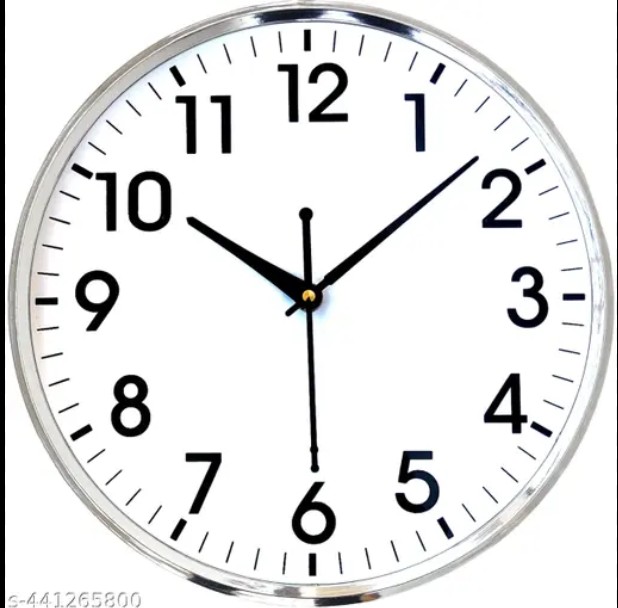
\includegraphics[width=2in]{Analog clock.png}\\
      we can have every value in the given limit.
        \end{center}
    \end{minipage}
    \begin{minipage}{0.5\linewidth}
        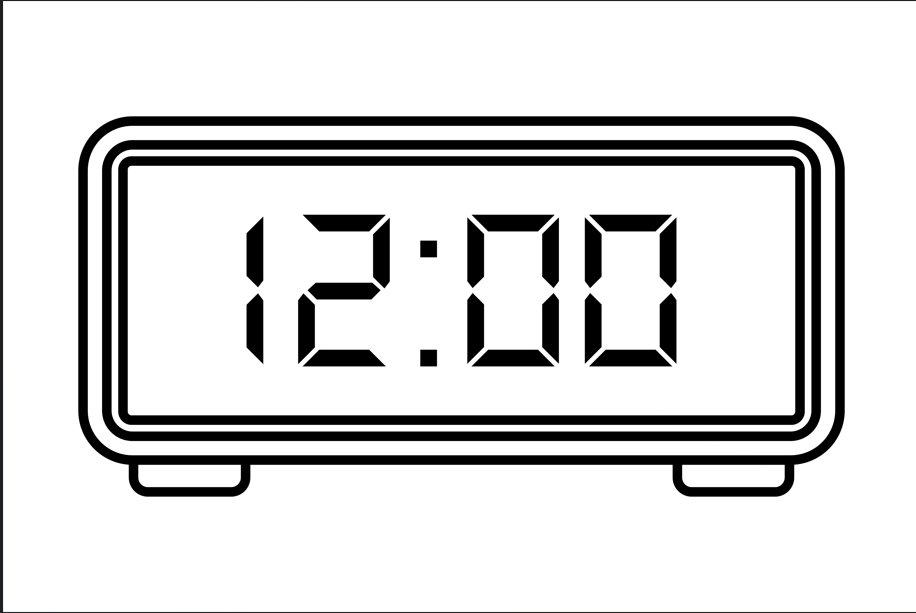
\includegraphics[width=2in]{Digital clock.png}\\
        In this clock we can't have 12:00:30 or 12:00:15.
    \end{minipage}

\end{questionbox}


\begin{center}
    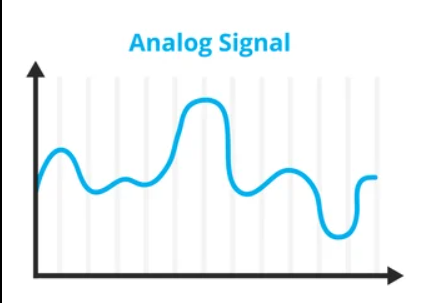
\includegraphics[scale=0.6]{Analog signal.png} \\
    Continuous Analog Signal
\end{center}
        

\vspace{10pt}

We can have every value in the given range.So this function called \textit{Analog signal.}
\par \textbf{Discrete Time Signal : } The signal which is defined for the discrete interval of time is called Discrete time signal.

\begin{figure}[h]
    \centering
    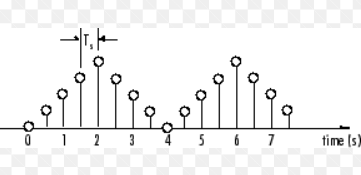
\includegraphics[width=0.5\textwidth]{Discrete time signal.png}
    \caption{Discrete time signal}
\end{figure}
\par From this graph we have the value at $t_0,t_1,t_2,......t_n$, but we can't have any value between $t_0$ and $t_1 $. Because we have monitored the function for the particular time.
\begin{enumerate}
    \item[*] Discrete time signal is the subset of analog signal.
    \item[*] All real life signal is analog signal.
\end{enumerate}
\underline{Example: }Sound,Temparature,Speed are analog signal.
\vspace{1em}
\par \textbf{Digital Signal : }A digital signal is a type of signal that represent data using discrete values,typically in the form of binary numbers (0s and 1s).Unlike analog signals which are continuous digital signals jumped between fixed level.\\
$\rightarrow$ In digital signals,we discrete both time and magnitude.\\
 $\rightarrow$ We divide the magnitude axis in to fixed number of levels and the signal can take value equal to these levels only.\\

% figure

\vspace{10pt}
For digital signal we have to make a level to minimize the error.\textcolor{red}{Increase the no of level reduce the error}.
\\ Again to minimize the value we have to take the lower value of the level. At $t_1$,$T$ is $9\degree C$.It is closer to $15\degree C$ but we can't take this value.We have to take $0\degree C$.\textbf{\textcolor{red}{The keypoint is we don't select the higher values ,we can just select the lower values. }}
\begin{questionbox}[What is the need of Digital Signal?]
$\rightarrow$ Digital signal is used in communication process to minimize the effect of noise(unwanted signals).

If the Analog signal voltage is $\left[0-5\right]\,V$ and we want to transmit this into $2.5\,V$.


%figure

But from this graph,there is no $2.7V$ level.So we can't take the voltage,we should take the lower level that is 2.5V.This the actual signal.This way Digital signal minimize the noise.
   
\end{questionbox}
\vspace{1em}

\section{Introduction of Digital Electronics}

\vspace{1em}

%figure


{\large Digital System $\longrightarrow$ Sub system $\longrightarrow$ Modules $\longrightarrow$ Basic Units(Logic gate) $\longrightarrow$ Circuit$\longrightarrow$ Transistor,Capacitor,Resistor.}
\vspace{1em}

\par \textbf{\large Switch and Bits intution }

\begin{enumerate}
    \item [$\blacksquare$] Advantage of Digital System : 
    \begin{enumerate}
        \item[(i)] Noise immunity.
        \item[(ii)] Uses less bandwith.
        \item [(iii)] Encryption.
        \item [(iv)] Efficiency for long distance transmission.
        \item [(v)] Accuracy.
    \end{enumerate}
    \item[*] If we want to increase the accuracy, we have to increase no. of level.
    \item [*] 
    \begin{enumerate}
        \item []n= no of levels
        \item []m= no of switch  
        $$\boxed{n=2^m}$$
    \end{enumerate}
    For 3 switch we have to need 8 levels for increasing accuracy.
    \\ In 2 bits number we have 4 possibility.
  
    %table
    
    \item[***]$\boxed{\text{no of bits = no of switch}}$ 
\end{enumerate}
\section{Introduction to Boolean Algebra}

\vspace{1em}
\begin{itemize}
  \item[$\longrightarrow$] It is the set of rules used to simplify the given logic expression without changing its functionality.
  \item[$\longrightarrow$] It is used when numbers of variables are less (like 1, 2, 3).
  \item[$\longrightarrow$] For more variables (like 4, 5, 6) we use another method which is known as \textbf{Map Methods}, also known as \textbf{Karnaugh Map or K-Map}.
\item Why do we minimize expression? $\longrightarrow$ To minimize gates.
  
\end{itemize}

\begin{questionbox}[What is Logic expression?]
 
    
\end{questionbox}
\textbf{\large Rules of Boolean algebra : }
\begin{enumerate}
    \item \textbf{Complement : } A complement = $\bar{A} \text{ or } A' \text{ (not A)}$
    \begin{enumerate}
        \item[*] $({A'})' = A$ \,\,\, [${0'}=1;\; {1'}=0$]
    \end{enumerate}
    \item \textbf{AND : }
    \begin{itemize}
        \item A.A=A
        \item A.0=0
        \item A.1=A
        \item A.{$A'$}=0
    \end{itemize}
    %TABLE

    \item \textbf{OR : }
    \begin{itemize}
        \item A+A=A
        \item A+0=A
        \item A+1=1
        \item A+$A'$=1
    \end{itemize}
    \item \textbf{Distributive Law : }
    \begin{itemize}
        \item A.(B+C)=AB+AC
        \item A+(B.C)=(A+B).(A+C)
        \item A+{$\bar{A}B$=A+B}
    \end{itemize}
    \item \textbf{Commutative Law : }
    \begin{itemize}
        \item A+B=B+A
        \item A.B=B.A
    \end{itemize}
    \item \textbf{Associative Law : }
    \begin{itemize}
        \item (A.B).C=A.(B.C)
    \end{itemize}
\end{enumerate}

\textcolor{red}{Priority : NOT $\rightarrow$ AND $\rightarrow$ OR.}
\vspace{1em}
\par {\large \textbf{Boolean Algebra Example : }}
\begin{examplebox}[Solve AB+A$B'$]
 Let 
\begin{align*}
      F&=AB+AB'\\
      &=A(B+B')\\
      &=A
\end{align*}
  
\end{examplebox}
\vspace{5pt}
\begin{examplebox}[Solve $AB+A\bar{B}C+A\bar{B}\bar{C}$]
    Let 
    \begin{align*}
        F &= AB+A\bar{B}C+A\bar{B}\bar{C}\\
        &= A[B+\bar{B}C+\bar{B}\bar{C}]\\
        &= A[B+\bar{B}(C+\bar{C)}]\\
        &=A[B+\bar{B}]=A
    \end{align*}
    
\end{examplebox}
\vspace{5pt}
\begin{examplebox}[Solve $(A+B+C)(A+\bar{B}+C)(A+B+\bar{C})$]
Let,
X=A+B
\begin{align*}
    F &=(A+B+C)(A+\bar{B}+C)(A+B+\bar{C}) \\ 
    &=(X+C)(A+\bar{B}+C)(X+\bar{C}) \\
    &=(X+C)(X+\bar{C})(A+\bar{B}+C) \\
    &=(X+C\bar{C})(A+\bar{B}+C)\\
    &=(X+0)(A+\bar{B}+C)\\
    &=(A+B)(A+\bar{B}+C)\\
    &=A+B(\bar{B}+C)\\
    &=A+BC=(A+B)(A+C)]\\
    &=A+B\bar{B}+BC=A+BC
\end{align*}
 
\end{examplebox}
\vspace{1em}

\section{Redundancy Theorem : }

\begin{enumerate}
    \item Three variable.
    \item Each variable is repeated twice.
    \item One variable is complimented
    \item Take the compliment variable.
\end{enumerate}
\begin{examplebox}[Simplify \ensuremath{Y = AB + A\bar{C} + BC}  ]
   
   \begin{align*}
   Y&=AB+\bar{A}C+BC\\
    &=AB+\bar{A}C+BC.1\\
    &=AB+\bar{A}C+BC(A+\bar{A})\\
    &=AB+\bar{A}C+\bar{A}BC+ABC\\
    &=AB(1+C)+\bar{A}C(1+B)\\
    &=AB+\bar{A}C
   \end{align*} 

\end{examplebox}
 \vspace{10pt}

 \begin{examplebox}[Simplify \ensuremath{F=AB+\bar{B}C+AC}]
    \begin{align*}
        F&=AB+B\bar{C}+AC\\
         &=AB+B\bar{C}+AC.1\\
         &=AB+B\bar{C}+AC(C+\bar{C})\\
         &=AB+ABC+B\bar{C}+A\bar{B}C\\
         &=AB(1+C)+B\bar{C}(1+A)\\
         &=AB+B\bar{C}
    \end{align*}
\underline{Short Cut:} The answer is the sum of  component without complement element  and the component with complement element.\\
 \end{examplebox}
\vspace{10pt}

\begin{examplebox}[Simplify \\
    \ensuremath{1.Y=A\bar{B}+BC+AC\\2.F=\bar{A}\bar{B}+A\bar{C}+\bar{B}\bar{C}}]
    \begin{minipage}{.5\linewidth}
         \begin{align*}
        1.Y&=A\bar{B}+BC+AC\\
           &=AC+A\bar{B}
    \end{align*}
    \end{minipage}
   \begin{minipage}{.5\linewidth}
        \begin{align*}
            2.F&=\bar{A}\bar{B}+A\bar{C}+\bar{B}\bar{C}\\
               &=\bar{A}\bar{B}+A\bar{C}
        \end{align*}
   \end{minipage}

\end{examplebox}
\vspace{10pt}
\begin{examplebox}[Simplify\\ \ensuremath{1.F=(A+B)(A+C)(\bar{B}+C)\\2.F=(A+B)+(\bar{A}+C)+(B+C)}]
   \begin{minipage}{.5\linewidth}
    \begin{align*}
          1.F&=(A+B)(A+C)(\bar{B}+C)\\
            &=(A+B)(\bar{B}+C)
    \end{align*}
   \end{minipage} 
   \begin{minipage}{.5\linewidth}
    \begin{align*}
        2.F&=(A+B)+(\bar{A}+C)+(B+C)\\
          &=(A+B)(\bar{A}+C)
    \end{align*}
   \end{minipage}
\end{examplebox}


\section{Sum of Product (SOP)}

SOP form only use for high function means o/p is 1.\\
Total no of Combination = $2^n$ \quad\quad [n$\rightarrow$ no of variables]\\
For 3 variables total combination=$2^3=8$\\[10PT]
\begin{minipage}{.5\linewidth}
    \begin{tabularx}{0.8\textwidth} { 
  | >{\centering\arraybackslash}X 
  | >{\centering\arraybackslash}X 
  | >{\centering\arraybackslash}X | }
 \hline
 \textbf{A} &  \textbf{B}& \textbf{F} \\
 \hline
  0 & 0& 0 \\
\hline
   0 & 0& 1 \\
\hline 
0 & 1& 0 \\
\hline
 0 & 1 & 1 \\
\hline
 1 & 0& 0 \\
\hline
 1 & 0& 1 \\
\hline
 1 & 1& 0 \\
\hline
 1 & 1& 1 \\
\hline
\end{tabularx}
\end{minipage}
\begin{minipage}{.5\linewidth}
    SOP form of this table :
    \begin{align*}
        F&=\bar{A}B\bar{C}+A\bar{B}\bar{C}+A\bar{B}C+ABC\\
         &=\sum m(2,4,5,6,7)
    \end{align*}
\end{minipage}

\vspace{10pt}
This particular form are called as standard or canonical SOP form and this is written directly form truth table.\\
Minterm $\rightarrow \bar{A}BC,ABC,AB,BC $ etc.\\
Maxterm $\rightarrow(A+B+C)$\\ [10pt]

\begin{examplebox}[Write the minimal SOP form of this function \\
    \ensuremath{F=\bar{A}B\bar{C}+A\bar{B}\bar{C}+A\bar{B}C+AB\bar{C}+ABC}]
    \begin{align*}
        F &=\bar{A}B\bar{C}+A\bar{B}\bar{C}+A\bar{B}C+AB\bar{C}+ABC\\
          &=\bar{A}B\bar{C}+A\bar{B}(\bar{C}+C)+AB(\bar{C}+C)\\
          &= \bar{A}B\bar{C}+A\bar{B}+AB\\
          &=\bar{A}B\bar{C}+A(\bar{B}+B)\\
          &=\bar{A}B\bar{C}+A\\
          &=A+B\bar{C}\quad\quad[\because A+\bar{A}B=A+B]
    \end{align*}
    This is the minimal SOP form of this cononical SOP form.

\end{examplebox}
\vspace{5pt}
 There are two types of SOP form.\\
 \textbf{1.standard/Cononical :} Each minterm is having all the variables in normal or complicated form.\\
 \underline{Example :} \(\bar{A}B+AB+\bar{A}\bar{B}\)\\
 \vspace{5pt}
 \textbf{2.Minimal :} Each minterm doesn't have all  the variables in normal or complicated form.\\
 \begin{questionbox}[For the given truth table minimize the SOP expression.]
    \begin{minipage}{.5\linewidth}
    \begin{tabularx}{0.8\textwidth} { 
  | >{\centering\arraybackslash}X 
  | >{\centering\arraybackslash}X 
  | >{\centering\arraybackslash}X | }
 \hline
 \textbf{A} &  \textbf{B}& \textbf{F} \\
 \hline
  0 & 0& 0 \\
\hline
   0 & 0& 1 \\
\hline 
0 & 1& 0 \\
\hline
 0 & 1 & 1 \\
 \hline
    \end{tabularx}   
    \end{minipage}
 \begin{minipage}{.4\linewidth}
    The cononical SOP form of this function \\
    \begin{align*}
        F&=\bar{A}B+AB\\
        &=B(\bar{A}+A)\\
        &=B
    \end{align*}
 \end{minipage}
 \end{questionbox}
 \vspace{10pt}
\begin{questionbox}[Simplify the expression for \ensuremath{Y=(A+B)=\sum (0,2,3)}]
    \begin{align*}
        Y &=M_0+M_2+M_3\\
          &=\bar{A}\bar{B}+A\bar{B}+AB\\
          &=\bar{B}(\bar{A}+A)+AB\\
          &=\bar{B}+AB\\
          &=A+\bar{B}
    \end{align*}
\end{questionbox}
\section{Product of Sum (POS form)}
$\rightarrow$ POS form is used for low function means the  O/P is '0'.\\
\begin{minipage}{.5\linewidth}
    \begin{align*}
        & 0\longrightarrow A\\
        & 1\longrightarrow \bar{A}\\
        & \text{POS form}
    \end{align*}
\end{minipage}
\begin{minipage}{0.05\linewidth}
        \rule{1pt}{2cm}
    \end{minipage}
    \begin{minipage}{.5\linewidth}
        \begin{align*}
            & 0 \longrightarrow \bar{A}\\
            & 1 \longrightarrow A\\
            & \text{SOP form}
        \end{align*}
        
    \end{minipage}
    \vspace{10pt}

    \begin{examplebox}[Write the minimize POS form of this truth table.]
        \begin{minipage}{.5\linewidth}
    \begin{tabularx}{0.8\textwidth} { 
  | >{\centering\arraybackslash}X 
  | >{\centering\arraybackslash}X 
  | >{\centering\arraybackslash}X  
  | >{\centering\arraybackslash}X| }
 \hline
 \textbf{A} &  \textbf{B}& \textbf{C} & \textbf{F}\\
 \hline
  0 & 0& 0 & 0\\
\hline
   0 & 0& 1 & 0\\
\hline 
0 & 1& 0 & 1 \\
\hline
 0 & 1 & 1 & 0\\
\hline
 1 & 0& 0 & 1 \\
\hline
 1 & 0& 1 & 1\\
\hline
 1 & 1& 0 & 1\\
\hline
 1 & 1& 1 & 1\\
\hline
\end{tabularx}
    \end{minipage}
    \begin{minipage}{.32\linewidth}
        \begin{align*}
            F&=(A+B+C).(A+B+\bar{C})(A+\bar{B}+\bar{C}) \rightarrow [\text{maxterm}]\\
            &=(X+C)(X+\bar{C})(A+\bar{B}+\bar{C})\\
            &=(X+C\bar{C})(A+\bar{B}+\bar{C})\\
            &=A+B(\bar{B}+\bar{C})\\
            &=A+B\bar{B}+B\bar{C}\\
            &=A+B\bar{C}\\
            &=(A+B)(A+C) \rightarrow [\text{Minimal POS form}]
        \end{align*}
    \end{minipage} 
    \end{examplebox}
    \vspace{10pt}
    \begin{questionbox}[For the given truth table minimize the POS form]
        \begin{minipage}{.5\linewidth}
    \begin{tabularx}{0.8\textwidth} { 
  | >{\centering\arraybackslash}X 
  | >{\centering\arraybackslash}X 
  | >{\centering\arraybackslash}X | }
 \hline
 \textbf{A} &  \textbf{B}& \textbf{Y} \\
 \hline
  0 & 0& 0 \\
\hline
   0 & 0& 1 \\
\hline 
0 & 1& 0 \\
\hline
 0 & 1 & 1 \\
 \hline
    \end{tabularx}   
    \end{minipage}
        \begin{minipage}{.32\linewidth}
            \begin{align*}
                Y&=(A+\bar{B})(\bar{A}+\bar{B})\\
                &=\bar{B}+A\bar{A}\\
                &=\bar{B}\\
                &\boxed{\prod (M_1,M_2)}=\prod M(1,3)=\sum M(0,2)\\
                & \qquad\qquad\qquad\qquad\quad \text{POS}\qquad\quad\quad\text{SOP}
            \end{align*}
        \end{minipage}
    \end{questionbox}
     \textcolor{red}{Important}\\
 \begin{itemize}
    \item SOP form $\longrightarrow $AND [more] $\rightarrow$ [If the equation has many AND gate,we use SOP]\\
    \item POS form $\longrightarrow$ OR [more] $\rightarrow \ $ [If the equation has many OR gate,we use POS]\\
 \end{itemize}
 \textbf{Example of some SOP and POS form}\\
 For those type of question, the truth table and equation are given.\\ 
 \begin{examplebox}[Minimize the equation\\
     \ensuremath{Y(A,B,C)=\sum M(0,2,3,6,7)\\Y(A,B,C)=\prod M(1,4,5)}]
    OR\\
     \begin{minipage}{.32\linewidth}
    \begin{tabularx}{0.5\textwidth} { 
  | >{\centering\arraybackslash}X 
  | >{\centering\arraybackslash}X 
  | >{\centering\arraybackslash}X  
  | >{\centering\arraybackslash}X| }
 \hline
 \textbf{A} &  \textbf{B}& \textbf{C} & \textbf{F}\\
 \hline
  0 & 0& 0 & 0\\
\hline
   0 & 0& 1 & 0\\
\hline 
0 & 1& 0 & 1 \\
\hline
 0 & 1 & 1 & 0\\
\hline
 1 & 0& 0 & 1 \\
\hline
 1 & 0& 1 & 1\\
\hline
 1 & 1& 0 & 1\\
\hline
 1 & 1& 1 & 1\\
\hline
\end{tabularx}
    \end{minipage}
    \begin{minipage}{.32\linewidth}
        \text{SOP}\\
        \begin{align*}
            Y&=\bar{A}\bar{B}\bar{C}+\bar{A}B\bar{C}+\bar{A}BC+AB\bar{C}+ABC\\
             &=\bar{A}\bar{B}\bar{C}+\bar{A}B(\bar{C}+C)+AB(\bar{C}+C)\\
             &=\bar{A}\bar{B}\bar{C}+\bar{A}B+AB\\
             &=\bar{A}\bar{B}\bar{C}+B(\bar{A}+A)\\
             &=\bar{A}\bar{B}\bar{C}+B\\
             &=B+\bar{A}\bar{C}
        \end{align*}
    \end{minipage}
    \begin{minipage}{.32\linewidth}
        \text{\centering POS}\\
        \begin{align*}
            Y&=(A+B+\bar{C})(\bar{A}+B+C)(\bar{A}+B+\bar{C})\\
            &=(A+B+\bar{C})(\bar{A}+B+C\bar{C})\\
            &=(A+B+\bar{C})(\bar{A}+B)\\
            &=B+(A+\bar{C})\bar{A}\\
            &=B+\bar{A}\bar{C}
        \end{align*}
    \end{minipage}
 \end{examplebox}


 \section{Minimal to Cononical form Conversion }

\par For SOP form$,$ \\
 \textbf{Step-1} Look at the variables and what the number of variables.\\
 \textbf{Step-2} Find missing variables.\\
 \textbf{Step-3} In the turm of missing variable we put this variable and its compliment.\\
 \textbf{Step-4} Ignore repeated part.\\

\vspace{5pt}
 For POS form$,$\\
 \textbf{Step-1} Look at the variables and what the number of variables.\\
 \textbf{Step-2} Find missing variables.\\
 \textbf{Step-3} Retrieve the absent variable.
 \begin{examplebox}[Convert this in cononical form \ensuremath{Y=A+\bar{B}C}]
    \begin{minipage}{0.5\linewidth}
        \begin{align*}
        Y&=A+\bar{B}C\\
        &=A.1.1+1.\bar{B}C\\
        &=A(B+\bar{B})(C+\bar{C})+(A+\bar{A})\bar{B}C\\
        &=ABC+AB\bar{C}+A\bar{B}C+A\bar{B}\bar{C}+A\bar{B}C+\bar{A}\bar{B}C\\
        &=ABC+AB\bar{C}+A\bar{B}C+A\bar{B}\bar{C}+\bar{A}\bar{B}C\\
    \end{align*}

    \end{minipage}
    
    \begin{minipage}{0.5\linewidth}
        \begin{align*}
            Y&= (A+B+\bar{C})(\bar{A}+C)\\
            &= (A+B+\bar{C})(\bar{A}+C+0)\\
            &=(A+B+\bar{C})(\bar{A}+C+B\bar{B})\\
            &=(A+B+\bar{C})(X+B\bar{B})\\
            &=(A+B+\bar{C})(X+B)(X+\bar{B})\\
            &=(A+B+\bar{C})(\bar{A}+B+C)(\bar{A}+\bar{B}+C)
        \end{align*}

    \end{minipage}
 \end{examplebox}
\vspace{10pt}
\begin{questionbox}[In a minimal SOP form\ensuremath{,}how many no of minterms in the logical expression \ensuremath{A+\bar{B}C} ]
    \begin{align*}
        F&=A+\bar{B}C\\
        &=A.1.1+1.\bar{B}C\\
        &=A(B+\bar{B})(C+\bar{C})+(A+\bar{A})\bar{B}C\\
        &=ABC+AB\bar{C}+A\bar{B}C+A\bar{B}\bar{C}+A\bar{B}C+\bar{A}\bar{B}C\\
        &=ABC+AB\bar{C}+A\bar{B}C+A\bar{B}\bar{C}+\bar{A}\bar{B}C\\
    \end{align*}
    No of  term=5
\end{questionbox}
\vspace{10pt}

\begin{questionbox}[With two variables\ensuremath{,}how many no of maximum  minterms and maxterms?]
    \begin{align*}
        A,B \longrightarrow 2^2=4\longrightarrow \text{Possible combination}.\\
        \text{For n variable}\longrightarrow 2^n=\text{Maxterms or Minterms}.
    \end{align*}
\end{questionbox}
\vspace{10pt}
\begin{questionbox}[For \ensuremath{n=4,}what is the total number of logical expression?]
    For n=2,
    %$$ (A,B)\longrightarrow \text{rows}=2^n=2^2=4\longrightarrow \text{Expressions}=2^{rows}=2^4=16$$
    %\bigg[ A \quad A\bar{B} \quad AB \\ A+B
    
\end{questionbox}
\end{document}